\documentclass[a4paper,10pt]{scrartcl}
\usepackage{physik-vorlesung}

\title{Experimentalphysik I}

\begin{document}

\maketitle

\tableofcontents

\newpage

\section*{Vorwort}
\begin{seg}{Ziele:}
\begin{itemize}
\item Experimentelle und theoretische Grundlagen der Newtonschen Mechanik, Wärmelehre, Thermodynamik
\item Als Einstieg möglichst auf sehr formale u. aufwendige Herleitungen verzichten, Grundprinzipien der Physik verdeutlichen
\item Veranschaulichung des Stoffs durch Demonstrationsexperimente in der Vorlesung
\item An physikalischen Beispielen werden die notwendige Bedingungen geklärt
\end{itemize}
\end{seg}

\begin{seg}{Ist Physik immer streng vorhersehbar?}
häufig ja, aber es gibt auch Ausnahmen:
\begin{itemize}
\item Wettervorhersage
\item \emph{chaotisches Pendel}
\item \emph{Galton-Brett}
\begin{figure}[h]
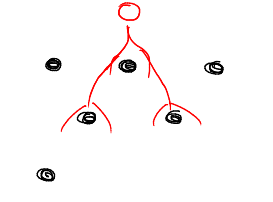
\includegraphics{fig1.png}
\end{figure}
\item \emph{Brownsche Bewegung}

\begin{figure}[h]
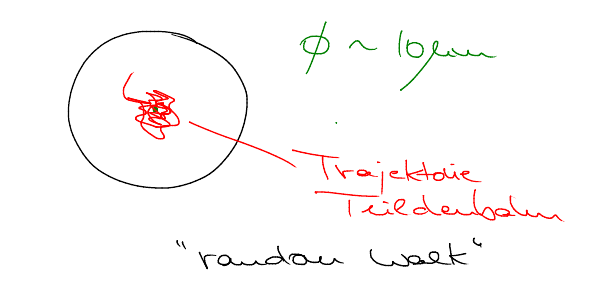
\includegraphics[scale=0.5]{fig2.png}
\end{figure}

\item \emph{Quantenmechanik}\\
Es gilt die Heisenbergsche Unschärferelation:
\[
\underbrace{\Delta x}_{\text{Ortsunschärfe}} \cdot \underbrace{\Delta p}_{\text{Impulsunschärfe}}
\]
\begin{figure}[h]
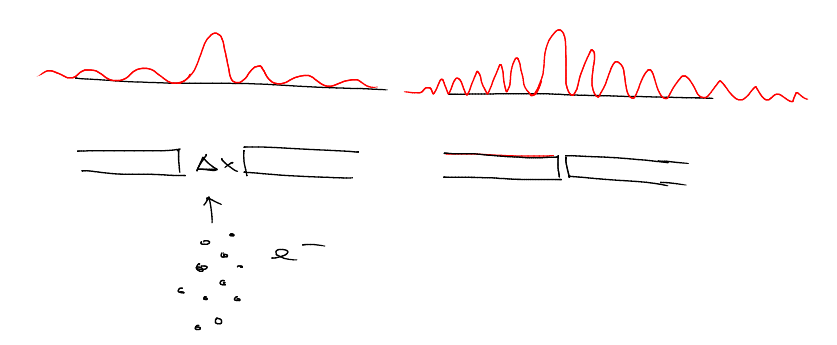
\includegraphics[scale=0.5]{fig3.png}
\end{figure}
\end{itemize}
\section{Physikalische Größen}
Eine \emph{Physikalische Größe} besteht aus einem \emph{Zahlenwert} und einer \emph{Einheit}.
\begin{ex*}
$1 \text{ in } \hat = \text{ Breite d. Daumens}$
Dies wurde später dann modifiziert, sodass die Einheit zur Länge drei aneinander liegenden Gerstenkörner umdefiniert worden ist.
\begin{figure}[h]
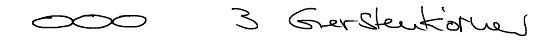
\includegraphics[scale=0.5]{fig4.png}
 \end{figure}
 
 Wünsche: wenige, aber überall nachprüfbare Einheiten $\rightarrow$ Basiseinheiten, Grundeinheiten
 \end{ex*}
 \end{seg}
 \subsection{Basiseinheiten}
 \begin{enumerate}[a]
\item Zeit \\
Die Grundeinheit der Zeit ist $1$ Sekunde(s).  Diese lässt sich definieren durch den Vergleich mit periodischen Vorgang. Es gilt:
\[
T=2\pi \sqrt{\frac{l}{g}}
\]

\[
l=24,8 \text{cm} \rightarrow T=1s
\]
\begin{itemize}
\item Quarzplättchen besitzen eine Frequenz aus dem $kHz$-Bereich.
\begin{figure}[h]
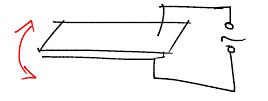
\includegraphics[scale=0.5]{fig5.png}
\end{figure}

Sie Besitzen einen Gangungenauigkeit von $1$ s/Woche. Sie besitzen also einen Fehler von $1$s pro $10^6$s
\item Es gibt aber auch die Möglichkeit mittels atomarer Eigenschwingungen (atomare Uhren) die Zeit noch genauer zu messen.  Deren Ganggenauigkeit entspricht $1$ s/$3000$ Jahren. Dies findet unter anderem Anwendung im GPS. 
\item $\ce{^{133}Cs}$ Hyperfeinübergang

Es ergibt sich die Definition $1\s=9.192.631.770$-faches der Periodendauer des Hyperfeinübergangs in $\ce{^{133}Cs}$. Diese ist überall nachvollziehbar!

\begin{seg}{Größenordungen von Zeiten}
\begin{table}[h]
\begin{tabular}{c r}
Weltall: & $10^8 \s$ \\
Mensch: & 1$10^9 s$ \\
Pulsschlag: & $1 s$ \\
Licht durchläuft $30 cm$: & $10^-9 s$ \\
Licht durchläuft Atom: & $10^-18 s$
\end{tabular}
\end{table}
Mit Hilfe von Präfixen kann man den Einheit eine neue Größenordnung geben. Hier die geläufigen Präfixe:

\begin{tabular}[h]
\begin{tabular}[c c c]
 $1\m$ & Milli & $10^{-3}$\\
 $1\my$ & Mikro $ 10^{-6}$\\
$1\nano$ & Nano $ 10^{-9}$ \\
$1\p$ & Piko & $ 10^{-12}$\\
$1\f$ & Fakto & $10^{-15}$\\
$1\a$ & Atte & $10^{-18}$\\
$1\k$ & Kilo & $10^3$ \\
$1\M$ & Mega & $10^6$ \\
$1\G$ & Giga & $10^9$ \\
$1\T$ & Terra & $10^12$ \\
$1\P$ & Peta & $10^15$ \\
$1\E$ & Exa & $10^18$
\end{tabular}
\end{table}
Zeitmessung durch radioaktiven Zerfall Kerne mit großer Masse $\rightarrow$ instabil $N=$ Zahl instabiler Kerne.
charakteristisch: $\frac{dN}{dt} ~ N(t)$
Wahrscheinlich, dass Kern zerfällt ist unabhänfig von allem anderen Kernen.
\begin{equation}
 \frac{dN}{dt}=-\lambda \cdot N(t), \qquad \lambda: \text{ Zerfallskonstanste}, \lambda>0
\end{equation}
\begin{equation}
 N(T)=N_0 \cdot e^{-\lambda t}, \qquad N_0:= N(0), [\lambda]=\frac{1}{s}
\end{equation}

\begin{figure}[h]
 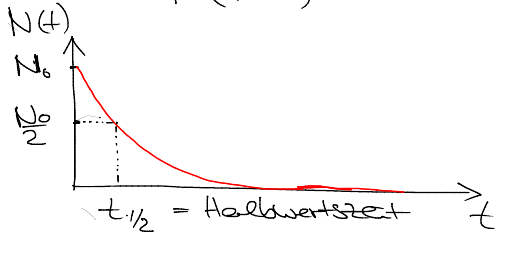
\includegraphics{fig6.png}
\end{figure}

\begin{align*}
 \frac N_0 2 &= N_0 \cdot e^{-\lambda t_{\frac 1 2}}}\\
 \ln 0.5&=-\lambda \cdot t_{\frac 1 2}\\
 t_{\frac 1 2} &= - \frac{\ln 0.5}\lambda = {\ln 2}{\lambda} 
\end{align*}
\begin{ex*}
 \begin{enumerate}[a)]
  \item $^{224}_{88} Tn \rightarrow ^{220}_{86} Ru + \alpha, \qquad \alpha=^4_2 He$ mit Halbwertszeit $t_{\frac 1 2}=556s$
  \item $\beta$-Zerfall: $^14_6 C \to ^14_7 N + e^-+\_ v_l$ mit Halbwertszeit $t_{\frac 1 2}=5730 a$  
\end{enumerate}
\end{seg}
\section*{Radio-Carbon-Methode}
Kohlenstoff: $^12_6 C, ^13_6 C, ^14_6 C$
Verteilung in Atmosphäre 
\[
 ^12 C:  98,89\%
 ^13 C: 1,11\%
^14 C: 10^-10 \%
\]
Wobei erstere beiden stabil und $^14 C$ instabil ist.  Lebende Organismen besitzen aufgrund von Stoffaustausche identische Kohlenstoff-Verteilung.  Stirbt der Organismus verändert sich Isotopenverhältnis.
\begin{align*}
 ^14 C(t)&=^14 C_0 \cdot e^{-\lambda t} \\
^13 C(t)&=^12 C_0\\
\frac{^14 C}{^12 C} |_\text{Fossil} (t)= frac{^14 C_0}{^12 C_0} e^{-\lambda t}, \qquad \lambda=1.121\cdot 10^-4 \frac{1}{a}
\end{align*}
\section*{C^14-Methode: experimentelle Bestimmung}
$\frac{^14  C}{^12 C}$ im Fossil (Massenspektrum) $\rightarrow$ Alter $t$ \rightarrow Alter + Höhlenzeichnung in S-Frankreich:  $15.500$ Jahre 
\end{ex*}




\end{itemize}
\item Länge

1799: $1 m \hat = \frac{1}{400000000}$ des durch Paris gehenden Großkreises ($40\cdot 10^3$ km) $\rightarrow$ Grundeinheit $1$ m

Urmeter: $Pt_90$ $Ir_10$

Seit 1983:
\[
 1m=\text{ Länge des Weges Weges, den Licht im Vakuum in $\frac{1}{299792485} s$ zurücklegt.}
\]

\section*{Größenordnungen und Längen}

\begin{tabular}[c|c}
 Fixstern & $4\cdot 10^16 m$\\
 Erde-Sonne & $1.5 \cdot 10^11 m$\\
Erdradius & $63 \cdot 10^6 m $\\
Sichtbares Licht (Wellenlänge) & $ 500\cdot 10^-9$ m \\
Atomdurchmesser & 10^-10  \\
Kerndurchmesser 10 ^-15
\end{tabular}
\section*{Messung von Abständen}
Triangulation:
\begin{figure}
 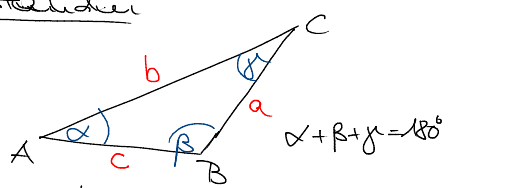
\includegraphics{fig7.png}
\end{figure}
Sinussatz: $\frac{c}{\sin\gamma} = \frac{a}{\sin{\beta}}=\frac{a}{\sin\alpha}$ \\
\begin{itemize}
 \item $\alpha, \beta$ bekannt $\to$ 
\end{itemize}
\section*{Abstand-Erde-Mond}
\begin{figure}[h]
 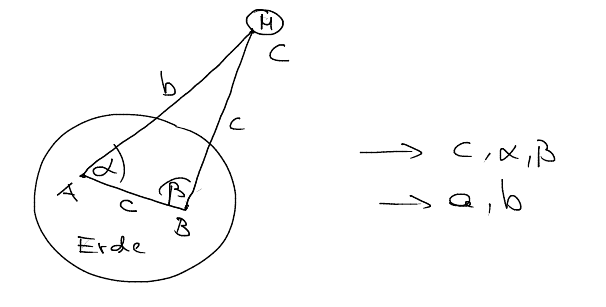
\includegraphics{fig8.png}
\end{figure}

\section*{Abstand Erde-Sonne}
Als Basis (c) wähle Erde-Mond
\begin{figure}
 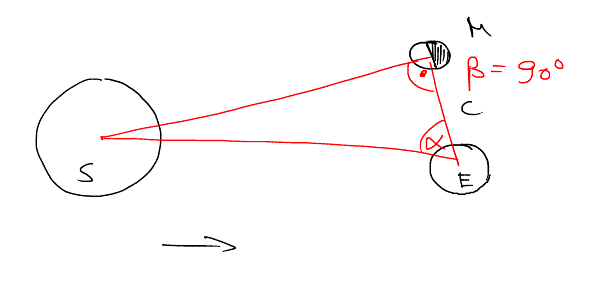
\includegraphics{fig9.png}
\end{figure}
Bei Halbmond besitzt $\beta=90^°$.  Den Abstand Erde-Mond lässt sich messen. Dann genügt es Den Winkel zwischen Mond und Sonne auf der Erde messen und damit ergibt sich der Abstand zum Mond.

\section*{LIDAR (Light Detection and raging)}
\begin{figure}[h]
 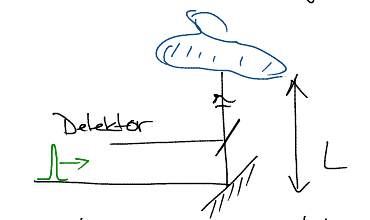
\includegraphics{fig10.png}
\end{figure}
\[
T=2L/c
\]

\section*{Messungen kleiner Entfernungen Laserinterferometer (Michelson-Int)}

\begin{figure}[h]
 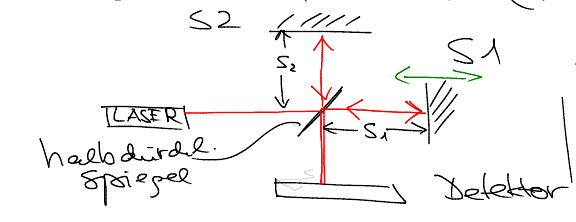
\includegraphics{fig11.png}
\end{figure}

\[
 \Delta s= 2 |s_1-s_2|
\]

Die Verschiebung um $\frac{20 \my m}{64 Maxima}=0.625 \to \lambda=630\my m $

\item Masse \\
Die Grundeinheit ist $1kg \hat = \text{Masse des Urkilogramms Zylinder\ Pt_{90}Ti_{10}

Vermutlich 2014:

\[
 1 Mol= 6022\cdot 10^23 \cdot ^28 Si \hat = 28.09 g
\]
\[
35,599 Mol ^28 Cr \hat = kg
\]
\[
$2,1441 \cdot 10^25 ^28 Si Atome \hat = 1 kg
\]

Zeit, Länge, Masse
SI


\end{enumerate}
\end{document}
